\documentclass[11pt]{article}
\usepackage[margin=1in]{geometry}
\usepackage{graphicx}
\usepackage{booktabs}
\usepackage{hyperref}
\hypersetup{colorlinks=true,linkcolor=blue,urlcolor=blue}
\title{Pre-ML Gating and Rolling Plan}
\author{TP2 SPY Call Pipeline}
\date{June 2026}
\begin{document}
\maketitle

\section*{Purpose}
The pre-ML gating step studies which parts of the conservative bid/ask TP2
universe are stable enough for model training. It is diagnostic: the final
paper result should use rolling out-of-sample evaluation rather than choosing a
single in-sample gate.

\section*{Active Strategy Families}
\begin{center}
\begin{tabular}{lrrrr}
\toprule
Strategy & Candidates & Valid rows & Net P\&L & Median return \\
\midrule
K1 & 228,241 & 107,326 & \$639.36M & -0.68\% \\
T1 & 228,241 & 106,636 & \$604.68M & -1.00\% \\
K2 & 228,241 & 106,636 & -\$53.56M & -1.44\% \\
T2 & 228,241 & 107,326 & -\$18.94M & -1.12\% \\
\bottomrule
\end{tabular}
\end{center}

\section*{Rolling Split}
The adopted rolling split is:
\[
\mathrm{train\ 3\ years} \rightarrow \mathrm{validate\ 1\ year}
\rightarrow \mathrm{test\ 1\ year}.
\]
The split is by episode signal date. Future labels, exit dates, realized P\&L,
and post-signal lifecycle rows are excluded from features.

\begin{figure}[h]
\centering
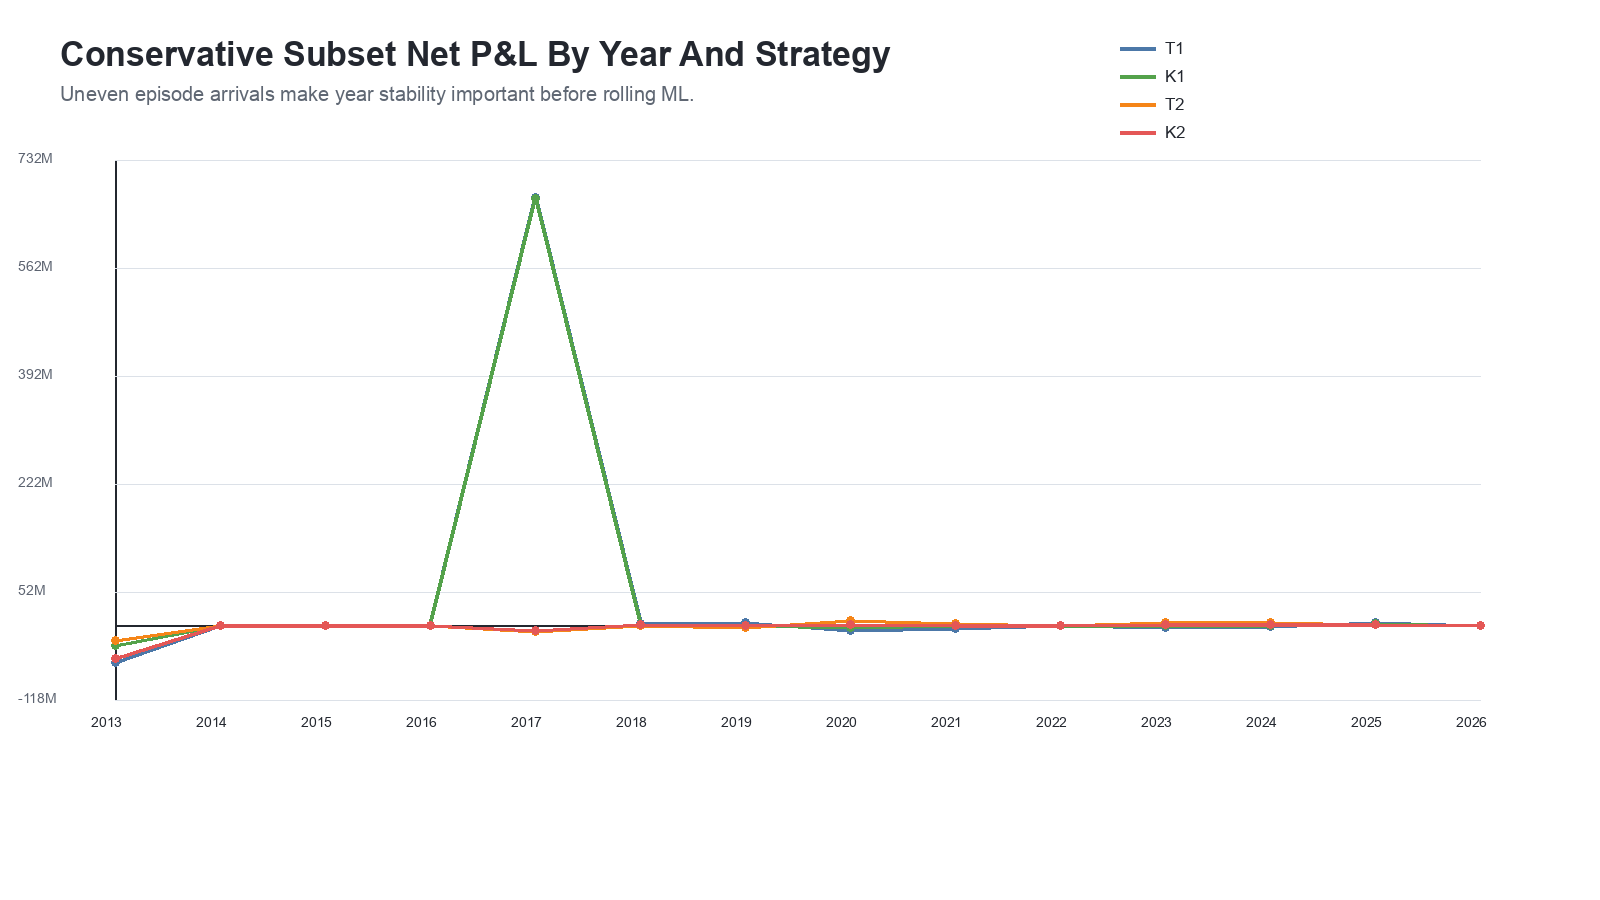
\includegraphics[width=\linewidth]{figures/pre_ml_strategy_year_stability.png}
\caption{Strategy-level year stability diagnostics.}
\end{figure}

\begin{figure}[h]
\centering
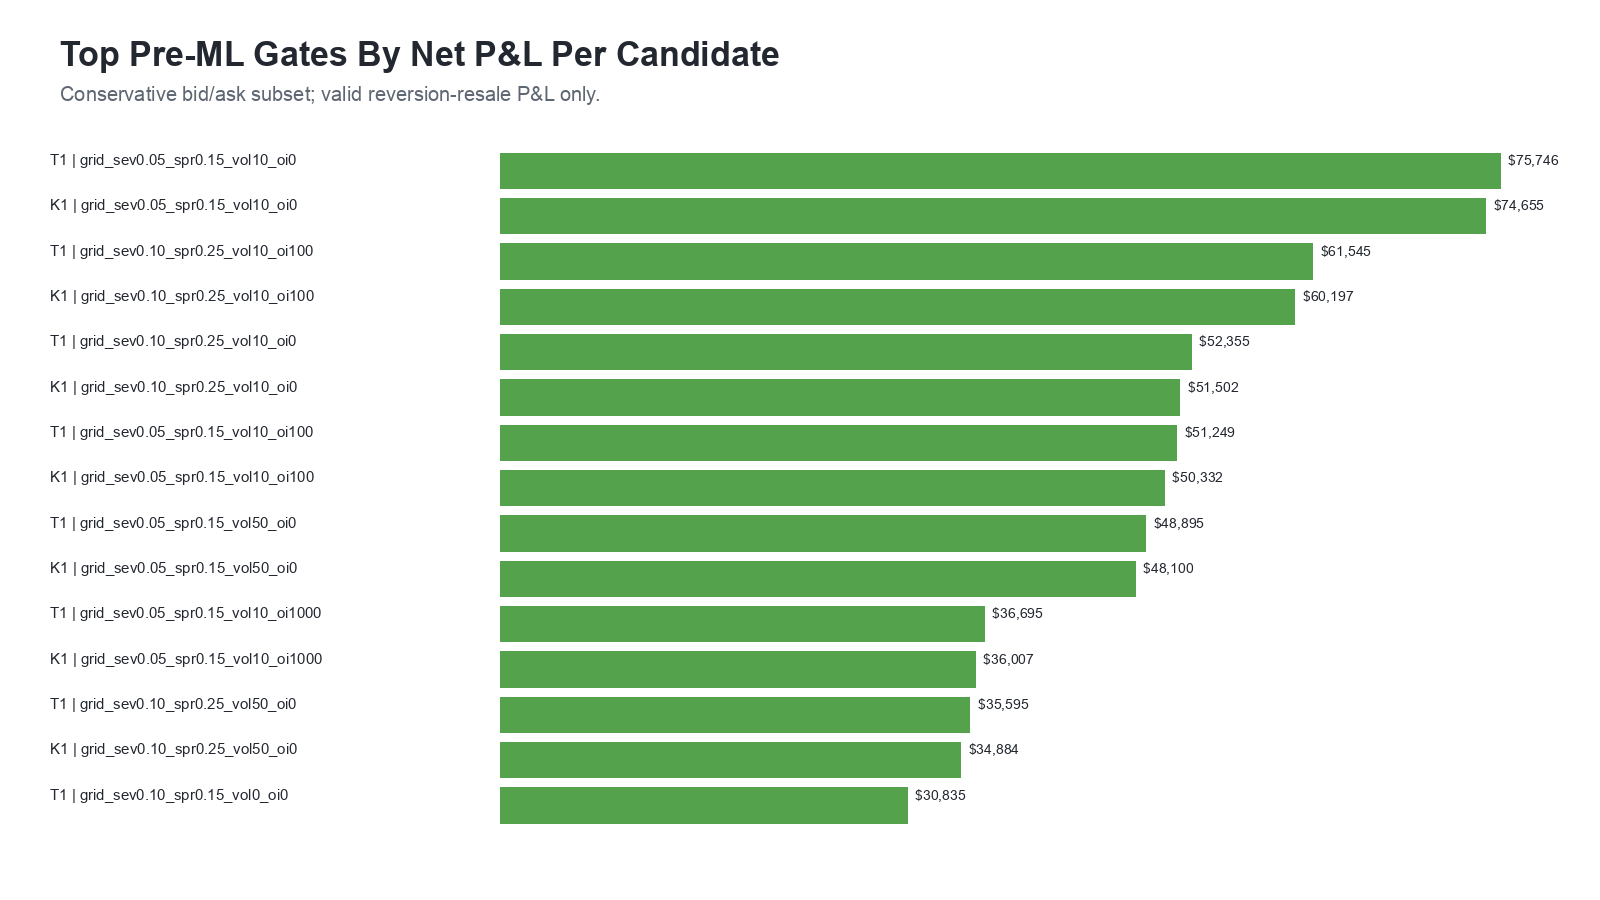
\includegraphics[width=\linewidth]{figures/pre_ml_top_gates_by_net_pnl_per_candidate.png}
\caption{Top gate diagnostics by net P\&L per candidate.}
\end{figure}

\section*{Interpretation}
Aggregate P\&L is positive for K1 and T1, but median returns are negative.
That means the opportunity is tail-driven and needs rolling ML, quality gates,
and concentration stress tests before being treated as a publishable trading
claim.

\end{document}
